As shown in Figure \ref{fig:turtlebot3}, the TurtleBot3 is equipped with many components, including a Raspberry Pi 4 (small computer) for onboard processing, a differential drive system, and a 360° 2D LiDAR sensor for observations. Due to the limitations of the onboard computer, the robot (client) relies on an external computer (server) for most processing tasks. The server processes data obtained by the robot's LiDAR sensor and transmits control parameters back to it at very fast regular intervals. These control parameters are the linear and angular velocities ($v,\omega$) of the robot that control the differential drive system. This driving system consists of two wheels, one on each side, that can be controlled independently, allowing the robot to turn by having one wheel turn more slowly than the other \parencite{corkeRoboticsVisionControl2023}. The LiDAR sensor, which constantly rotates to observe around the robot, measures distances by ``[emitting] short pulses of infrared laser light and [measuring] the time for the reflected pulses to return'' \parencite{corkeRoboticsVisionControl2023}.

\begin{figure}[!htb]
    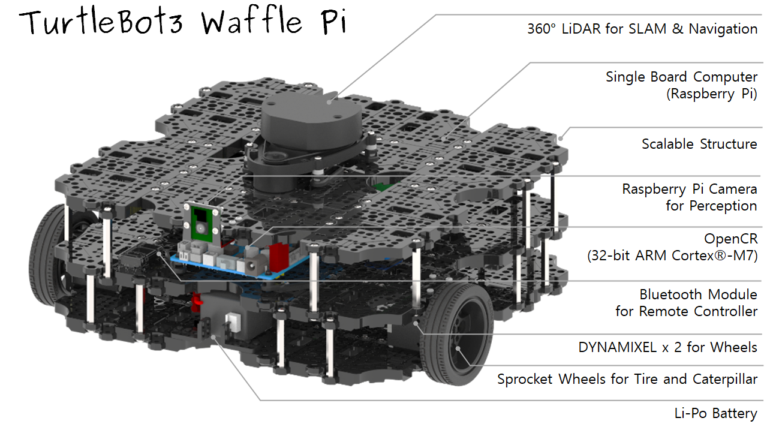
\includegraphics[width=8cm]{turtlebot3.png}
    \centering
    \caption{Components of the TurtleBot3 Waffle Pi \parencite{ROBOTISEManual}.}
    \label{fig:turtlebot3}
\end{figure}

A few essential pieces of software are used for the development of the robot. Firstly, as ROS2 Humble best supports the Ubuntu 22.04 LTS (Jammy Jellyfish) Linux distribution, this operating system is used to code and control the robot \parencite{InstallationROSDocumentation}. The use of ROS2 allows the robot to be programmed using a combination of both Python and C++. Secondly, Gazebo Ignition Fortress is used to simulate and visualize the robot in a 3D environment. This allows writing and testing on a virtual robot without the need for real robot hardware, which facilitates collaboration between students and remote development. Thirdly, RViz is used to control the robot and visualize the cost map.